\documentclass[10pt]{beamer}

\newcommand{\lectnum}{L05}
\newcommand{\lecttitle}{Neural Networks: \\ CNNs, RNNs, and Transformers}

\usepackage{amsmath, amssymb, graphicx}
\usepackage[]{algorithm2e}
\usepackage{pdfpages}
\usepackage{bm}
\usepackage{relsize}
\usepackage[british]{babel}
\usepackage{tikz,tikzsymbols}
\usepackage{hyperref}
\usepackage{cancel}
\usepackage{caption,subcaption}
\usepackage{adjustbox}
\usepackage{overpic}
\usepackage[UKenglish]{isodate}

\usetikzlibrary{arrows,decorations.markings,decorations.pathreplacing,positioning}

\newcommand{\bs}{\boldsymbol}


\hypersetup{colorlinks,linkcolor=,urlcolor=blue}
\newenvironment{titledslide}[1]{\begin{frame}\frametitle{#1}}{\end{frame}}

\mode<presentation>{\setbeamercovered{transparent}}

\setbeamertemplate{sidebar right}{}
\setbeamertemplate{footline}{%
\hfill\usebeamertemplate***{navigation symbols}
\hspace{0.4cm}\lectnum: \insertframenumber{}/\inserttotalframenumber \hspace*{0.4cm}}

\author{Mengyan Zhang}

\title{COMS20018, Introduction to AI:\\ \vspace{5pt} \lecttitle}

\institute{School of Computer Science\\University of Bristol}
\date{5th October 2026}

%%%%%%%%%%%%%%%%%%%%%%%%%%%%%%%%%%%%%%%%%%%%%%%%%%%%%%%%%%%%%%%%%%%%%%

% colours from J. Alammar's Illustrated Transformer figures (darkened for projection)
\definecolor{aQ}{RGB}{175,60,210}
\definecolor{aK}{RGB}{235,125,0}
\definecolor{aV}{RGB}{40,130,230}
\definecolor{aS}{RGB}{150,150,0}
\definecolor{aZ}{RGB}{225,60,140}
\begin{document}
%%%%%%%%%%%%%%%%%%%%%%%%%%%%%%%%%%%%%%%%%%%%%%%%%%%%%%%%%%%%%%%%%%%%%%

\begin{frame}[fragile]
  \begin{tikzpicture}[remember picture, overlay]
    \node[anchor=north west, xshift=0.4cm, yshift=-0.4cm] at (current page.north west)
      {
\includegraphics[width=3.4cm]{figures/uob_logo.png}};
  \end{tikzpicture}
  \titlepage
\end{frame}
%%%%%%%%%%%%%%%%%%%%%%%%%%%%%%%%%%%%%%%%%%%%%%%%%%%%%%%%%%%%%%%%%%%%%%
\begin{frame}[fragile]

  \frametitle{Agenda}
  \begin{itemize}
  \item A short history, and the different shapes of data
  \item Images: convolutional networks (CNNs)
  \item Sequences: recurrent networks (RNNs), Attention and the Transformer
  \end{itemize}

  \vspace{6pt}
  \begin{itemize}
  \item[$\Rightarrow$] For each: \emph{what was it built for}, \emph{what
    problem did it address}, and \emph{where is it used}? 
  \end{itemize}

\end{frame}
%%%%%%%%%%%%%%%%%%%%%%%%%%%%%%%%%%%%%%%%%%%%%%%%%%%%%%%%%%%%%%%%%%%%%%
\begin{frame}[fragile]
\frametitle{A short history of neural network architectures}

\vspace{8pt}
\centerline{%
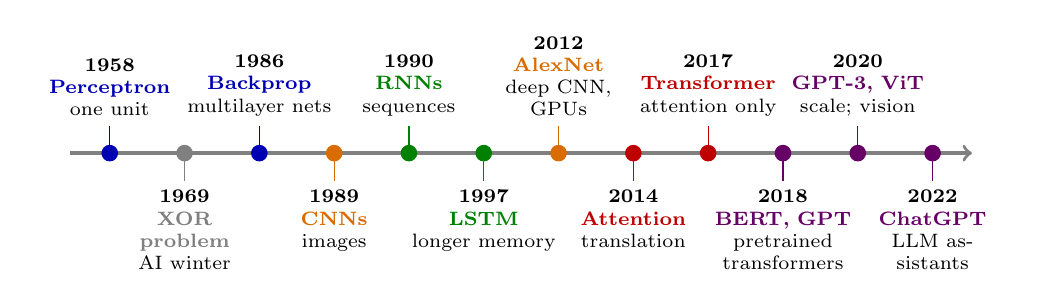
\begin{tikzpicture}
  \draw[->,very thick,gray] (-0.5,0) -- (10.95,0);
  \fill[blue!70!black] (0.00,0) circle (3pt);
  \draw[blue!70!black] (0.00,0) -- (0.00,0.35);
  \node[above=0.35cm,align=center,font=\scriptsize,text width=1.85cm] at (0.00,0) {\textbf{1958}\\{\color{blue!70!black}\textbf{Perceptron}}\\one unit};
  \fill[gray] (0.95,0) circle (3pt);
  \draw[gray] (0.95,0) -- (0.95,-0.35);
  \node[below=0.35cm,align=center,font=\scriptsize,text width=1.85cm] at (0.95,0) {\textbf{1969}\\{\color{gray}\textbf{XOR problem}}\\AI winter};
  \fill[blue!70!black] (1.90,0) circle (3pt);
  \draw[blue!70!black] (1.90,0) -- (1.90,0.35);
  \node[above=0.35cm,align=center,font=\scriptsize,text width=1.85cm] at (1.90,0) {\textbf{1986}\\{\color{blue!70!black}\textbf{Backprop}}\\multilayer nets};
  \fill[orange!85!black] (2.85,0) circle (3pt);
  \draw[orange!85!black] (2.85,0) -- (2.85,-0.35);
  \node[below=0.35cm,align=center,font=\scriptsize,text width=1.85cm] at (2.85,0) {\textbf{1989}\\{\color{orange!85!black}\textbf{CNNs}}\\images};
  \fill[green!50!black] (3.80,0) circle (3pt);
  \draw[green!50!black] (3.80,0) -- (3.80,0.35);
  \node[above=0.35cm,align=center,font=\scriptsize,text width=1.85cm] at (3.80,0) {\textbf{1990}\\{\color{green!50!black}\textbf{RNNs}}\\sequences};
  \fill[green!50!black] (4.75,0) circle (3pt);
  \draw[green!50!black] (4.75,0) -- (4.75,-0.35);
  \node[below=0.35cm,align=center,font=\scriptsize,text width=1.85cm] at (4.75,0) {\textbf{1997}\\{\color{green!50!black}\textbf{LSTM}}\\longer memory};
  \fill[orange!85!black] (5.70,0) circle (3pt);
  \draw[orange!85!black] (5.70,0) -- (5.70,0.35);
  \node[above=0.35cm,align=center,font=\scriptsize,text width=1.85cm] at (5.70,0) {\textbf{2012}\\{\color{orange!85!black}\textbf{AlexNet}}\\deep CNN, GPUs};
  \fill[red!75!black] (6.65,0) circle (3pt);
  \draw[red!75!black] (6.65,0) -- (6.65,-0.35);
  \node[below=0.35cm,align=center,font=\scriptsize,text width=1.85cm] at (6.65,0) {\textbf{2014}\\{\color{red!75!black}\textbf{Attention}}\\translation};
  \fill[red!75!black] (7.60,0) circle (3pt);
  \draw[red!75!black] (7.60,0) -- (7.60,0.35);
  \node[above=0.35cm,align=center,font=\scriptsize,text width=1.85cm] at (7.60,0) {\textbf{2017}\\{\color{red!75!black}\textbf{Transformer}}\\attention only};
  \fill[violet!80!black] (8.55,0) circle (3pt);
  \draw[violet!80!black] (8.55,0) -- (8.55,-0.35);
  \node[below=0.35cm,align=center,font=\scriptsize,text width=1.85cm] at (8.55,0) {\textbf{2018}\\{\color{violet!80!black}\textbf{BERT, GPT}}\\pretrained transformers};
  \fill[violet!80!black] (9.50,0) circle (3pt);
  \draw[violet!80!black] (9.50,0) -- (9.50,0.35);
  \node[above=0.35cm,align=center,font=\scriptsize,text width=1.85cm] at (9.50,0) {\textbf{2020}\\{\color{violet!80!black}\textbf{GPT-3, ViT}}\\scale; vision};
  \fill[violet!80!black] (10.45,0) circle (3pt);
  \draw[violet!80!black] (10.45,0) -- (10.45,-0.35);
  \node[below=0.35cm,align=center,font=\scriptsize,text width=1.85cm] at (10.45,0) {\textbf{2022}\\{\color{violet!80!black}\textbf{ChatGPT}}\\LLM assistants};
\end{tikzpicture}}

\vspace{6pt}
\begin{itemize}
\item Each step answered a limitation of the previous one, and the
  \emph{shape of the data} (grid, sequence) drove the design.
% \item[$\Rightarrow$] All are trained the same way: backpropagation.
%   Only the \emph{wiring} changes.
\end{itemize}

\end{frame}
%%%%%%%%%%%%%%%%%%%%%%%%%%%%%%%%%%%%%%%%%%%%%%%%%%%%%%%%%%%%%%%%%%%%%%
\begin{frame}[fragile]
\frametitle{Data comes in different shapes}

\vspace{2pt}
\centerline{%
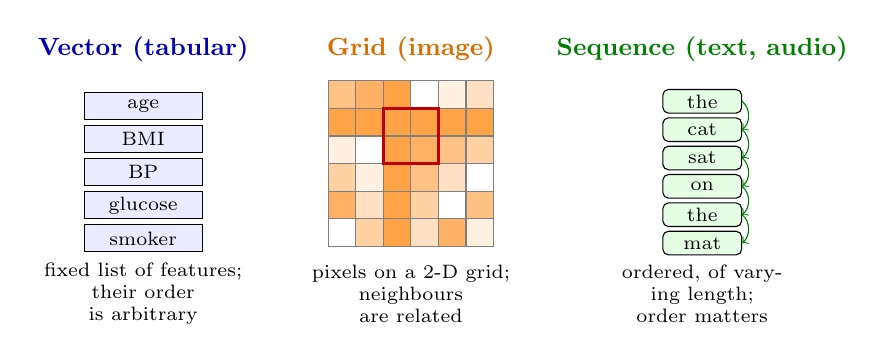
\begin{tikzpicture}[font=\scriptsize]
  % --- tabular / vector
  \begin{scope}[shift={(0,0)}]
    \node[font=\small\bfseries,blue!70!black] at (1.2,3.05) {Vector (tabular)};
    \foreach \v [count=\i] in {age,BMI,BP,glucose,smoker} {
      \node[draw,fill=blue!8,inner sep=1pt,minimum width=1.5cm,minimum height=0.34cm] at (1.2,2.75-0.42*\i) {\v};
    }
    \node[align=center,text width=2.7cm] at (1.2,-0.05) {\hyphenpenalty=10000 fixed list of features;\\their order is arbitrary};
  \end{scope}
  % --- grid / image
  \begin{scope}[shift={(3.4,0)}]
    \node[font=\small\bfseries,orange!85!black] at (1.2,3.05) {Grid (image)};
    \foreach \x in {0,...,5} \foreach \y in {0,...,5} {
      \pgfmathsetmacro{\c}{int(mod(3*\x+5*\y+\x*\y,7))*12}
      \fill[orange!\c!white] (0.15+0.35*\x,0.55+0.35*\y) rectangle ++(0.35,0.35);
    }
    \draw[gray,step=0.35,shift={(0.15,0.55)}] (0,0) grid (2.1,2.1);
    \draw[red!75!black,very thick] (0.85,1.6) rectangle ++(0.7,0.7);
    \node[align=center,text width=2.7cm] at (1.2,-0.05) {pixels on a 2-D grid;\\neighbours are related};
  \end{scope}
  % --- sequence
  \begin{scope}[shift={(6.7,0)}]
    \node[font=\small\bfseries,green!50!black] at (1.6,3.05) {Sequence (text, audio)};
    \foreach \w [count=\i] in {the,cat,sat,on,the,mat} {
      \node[draw,rounded corners=2pt,fill=green!10,inner sep=1pt,minimum width=1.0cm,minimum height=0.30cm] (w\i) at (1.6,2.75-0.36*\i) {\w};
    }
    \foreach \i [evaluate=\i as \j using int(\i+1)] in {1,...,5} \draw[->,green!50!black] (w\i.east) to[bend left=50] (w\j.east);
    \node[align=center,text width=2.9cm] at (1.6,-0.05) {ordered, of varying length;\\order matters};
  \end{scope}
\end{tikzpicture}}

\vspace{4pt}
{\small
\begin{tabular}{@{}lll@{}}
\textbf{Shape} & \textbf{Examples} & \textbf{Architecture}\\\hline
vector  & patient records, sensor readings & fully connected network\\
grid    & photos, X-rays, satellite images & {\color{orange!85!black}\textbf{CNN}}\\
sequence & sentences, speech, DNA & {\color{green!50!black}\textbf{RNN/LSTM}} $\to$ {\color{red!75!black}\textbf{Transformer}}\\
\end{tabular}}

% \vspace{4pt}
% \begin{itemize}
% \item[$\Rightarrow$] A \textbf{fully connected} network (every hidden unit
%   connected to every input) treats the input as a flat list: it ignores
%   that neighbouring pixels, or consecutive words, belong together. Each new
%   architecture builds that structure into its wiring.
% \end{itemize}

\end{frame}
%%%%%%%%%%%%%%%%%%%%%%%%%%%%%%%%%%%%%%%%%%%%%%%%%%%%%%%%%%%%%%%%%%%%%%
\begin{frame}[fragile]
\frametitle{Images: why a fully connected network struggles}

\centerline{%
\begin{tikzpicture}[font=\scriptsize]
  % image: a real MNIST digit
  \node[inner sep=0pt,anchor=south west] at (0,0) {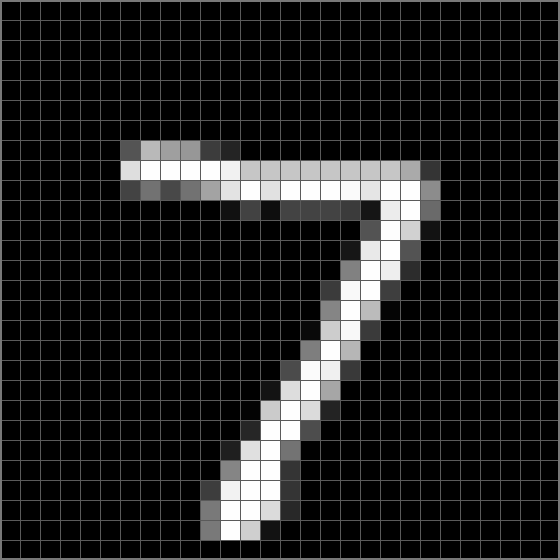
\includegraphics[width=2.1cm]{figures/mnist_digit7.png}};
  \node[below] at (1.05,0) {$28\times28$ pixels};
  \node[above,align=center] at (1.05,2.1) {one number per pixel\\(brightness 0--255)};
  % flatten arrow
  \draw[->,thick] (2.3,1.35) -- node[above]{flatten} (3.3,1.35);
  % inputs
  \foreach \y/\l in {2.1/$x_1$,1.6/$x_2$,1.1/$x_3$,0.0/$x_{784}$} {
    \node[draw,circle,fill=gray!20,inner sep=1pt,minimum size=0.42cm] (i\l) at (4.2,\y) {};
    \node[left] at (3.95,\y) {\l};
  }
  \node at (4.2,0.6) {$\vdots$};
  % hidden
  \foreach \y [count=\k] in {1.9,1.3,0.2} \node[draw,circle,fill=blue!70!black!20,inner sep=1pt,minimum size=0.42cm] (h\k) at (6.4,\y) {};
  \node at (6.4,0.8) {$\vdots$};
  \foreach \a in {2.1,1.6,1.1,0.0} \foreach \b in {1.9,1.3,0.2} \draw[gray] (4.41,\a) -- (6.19,\b);
  \node[below,align=center] at (4.2,-0.3) {784 inputs};
  \node[below,align=center] at (6.4,-0.3) {100 hidden units};
  \node[right,align=left] at (6.8,1.05) {every hidden unit\\has a weight to\\\emph{every} pixel};
\end{tikzpicture}}

\vspace{2pt}
{\small
\begin{itemize}
\item \textbf{Too many weights.} 
% $28 \times 28 = 784$ inputs, each wired to
%   100 hidden units: $784 \times 100 = 78{,}400$ weights. A $224\times224$
%   colour photo: $\approx$150,000 inputs; 1000 hidden units $\Rightarrow$
%   \textbf{150 million} weights.
\item \textbf{Layout is lost.} Flattening is like putting the photo through
  a paper shredder: which pixels were neighbours must be re-learned
\item[$\Rightarrow$] Two ideas fix both: \textbf{local patterns matter}
  (look at small patches), and \textbf{a pattern is the same wherever it
  appears} (reuse one detector everywhere).
\end{itemize}}

\vspace{-2pt}
{\fontsize{6}{6}\selectfont Image: a handwritten ``7'' from the MNIST dataset (LeCun, Cortes \& Burges), CC BY-SA 3.0.\par}

\end{frame}
%%%%%%%%%%%%%%%%%%%%%%%%%%%%%%%%%%%%%%%%%%%%%%%%%%%%%%%%%%%%%%%%%%%%%%
\begin{frame}[fragile]
\frametitle{Convolution (1/2): sliding a filter}

\begin{itemize}
\item \textbf{Convolution}: slide a small \textbf{filter} (also called a
  \textbf{kernel}) over the image. 
  % At each position, multiply the overlapping numbers and add them up: one
  % number of the \textbf{feature map}.
\end{itemize}

\vspace{2pt}
\centerline{\resizebox{0.72\textwidth}{!}{%
\begin{tikzpicture}[scale=0.62,every node/.style={font=\small}]
  \node at (0.5,3.5) {1};
  \node at (1.5,3.5) {0};
  \node at (2.5,3.5) {2};
  \node at (3.5,3.5) {1};
  \node at (0.5,2.5) {3};
  \node at (1.5,2.5) {1};
  \node at (2.5,2.5) {0};
  \node at (3.5,2.5) {2};
  \node at (0.5,1.5) {0};
  \node at (1.5,1.5) {2};
  \node at (2.5,1.5) {1};
  \node at (3.5,1.5) {0};
  \node at (0.5,0.5) {1};
  \node at (1.5,0.5) {0};
  \node at (2.5,0.5) {3};
  \node at (3.5,0.5) {1};
  \draw[step=1,gray] (0,0) grid (4,4);
  \node[orange!85!black] at (6.0,2.5) {\textbf{1}};
  \node[orange!85!black] at (7.0,2.5) {\textbf{0}};
  \node[orange!85!black] at (6.0,1.5) {\textbf{0}};
  \node[orange!85!black] at (7.0,1.5) {\textbf{1}};
  \fill[orange!85!black!15] (5.5,1) rectangle (7.5,3);
  \node[orange!85!black] at (6.0,2.5) {\textbf{1}};
  \node[orange!85!black] at (7.0,2.5) {\textbf{0}};
  \node[orange!85!black] at (6.0,1.5) {\textbf{0}};
  \node[orange!85!black] at (7.0,1.5) {\textbf{1}};
  \draw[step=1,gray,shift={(5.5,0)}] (0,1) grid (2,3); \draw[orange!85!black,very thick] (5.5,1) rectangle (7.5,3);
  \draw[step=1,gray,shift={(9,0.5)}] (0,0) grid (3,3);
  \only<1>{\fill[blue!70!black!20] (0,2) rectangle (2,4);  \fill[blue!70!black!25] (9.0,2.5) rectangle (10.0,3.5);}
  \only<2>{\fill[blue!70!black!20] (1,2) rectangle (3,4);  \fill[blue!70!black!25] (10.0,2.5) rectangle (11.0,3.5);}
  \only<3>{\fill[blue!70!black!20] (2,2) rectangle (4,4);  \fill[blue!70!black!25] (11.0,2.5) rectangle (12.0,3.5);}
  \node at (0.5,3.5) {1};
  \node at (1.5,3.5) {0};
  \node at (2.5,3.5) {2};
  \node at (3.5,3.5) {1};
  \node at (0.5,2.5) {3};
  \node at (1.5,2.5) {1};
  \node at (2.5,2.5) {0};
  \node at (3.5,2.5) {2};
  \node at (0.5,1.5) {0};
  \node at (1.5,1.5) {2};
  \node at (2.5,1.5) {1};
  \node at (3.5,1.5) {0};
  \node at (0.5,0.5) {1};
  \node at (1.5,0.5) {0};
  \node at (2.5,0.5) {3};
  \node at (3.5,0.5) {1};
  \draw[step=1,gray] (0,0) grid (4,4);
  \visible<1->{\node at (9.5,3.0) {2};}
  \visible<2->{\node at (10.5,3.0) {0};}
  \visible<3->{\node at (11.5,3.0) {4};}
  \visible<4->{\node at (9.5,2.0) {5};}
  \visible<4->{\node at (10.5,2.0) {2};}
  \visible<4->{\node at (11.5,2.0) {0};}
  \visible<4->{\node at (9.5,1.0) {0};}
  \visible<4->{\node at (10.5,1.0) {5};}
  \visible<4->{\node at (11.5,1.0) {2};}
  \only<1>{\draw[blue!70!black,very thick] (0,2) rectangle (2,4); \draw[blue!70!black,very thick] (9.0,2.5) rectangle (10.0,3.5);}
  \only<2>{\draw[blue!70!black,very thick] (1,2) rectangle (3,4); \draw[blue!70!black,very thick] (10.0,2.5) rectangle (11.0,3.5);}
  \only<3>{\draw[blue!70!black,very thick] (2,2) rectangle (4,4); \draw[blue!70!black,very thick] (11.0,2.5) rectangle (12.0,3.5);}
  \node at (4.75,2) {\Large $\ast$}; \node at (8.25,2) {\Large $=$};
  \node at (2,-0.55) {input image}; \node at (6.5,0.45) {filter}; \node at (10.5,-0.05) {feature map};
\end{tikzpicture}}}

\vspace{4pt}
\centerline{\small \only<1>{$1\cdot{\color{orange!85!black}1} + 0\cdot{\color{orange!85!black}0} + 3\cdot{\color{orange!85!black}0} + 1\cdot{\color{orange!85!black}1} = \mathbf{2}$}\only<2>{$0\cdot{\color{orange!85!black}1} + 2\cdot{\color{orange!85!black}0} + 1\cdot{\color{orange!85!black}0} + 0\cdot{\color{orange!85!black}1} = \mathbf{0}$}\only<3>{$2\cdot{\color{orange!85!black}1} + 1\cdot{\color{orange!85!black}0} + 0\cdot{\color{orange!85!black}0} + 2\cdot{\color{orange!85!black}1} = \mathbf{4}$}\only<4>{\dots\ and so on, sliding over \emph{every} position}}

\vspace{4pt}
\begin{itemize}
\item[$\Rightarrow$] The \emph{same} 4 filter weights are reused at every
  position (\textbf{weight sharing}); each output looks only at a small patch
  (\textbf{local receptive field}).
\item The filter's numbers are \textbf{weights}: they start random and are
  \emph{learned} by backpropagation, not designed by hand.
\end{itemize}

\end{frame}
%%%%%%%%%%%%%%%%%%%%%%%%%%%%%%%%%%%%%%%%%%%%%%%%%%%%%%%%%%%%%%%%%%%%%%
\begin{frame}[fragile]
\frametitle{Pooling: shrinking the feature maps}

\begin{itemize}
\item \textbf{Max pooling}: slide a $2\times2$ window over a feature map and
  keep only the \emph{largest} value in each window.
\end{itemize}

\vspace{2pt}
\centerline{\resizebox{0.5\textwidth}{!}{%
\begin{tikzpicture}[scale=0.62,every node/.style={font=\small}]
  \only<1>{\fill[blue!70!black!20] (0,1) rectangle (2,3); \fill[blue!70!black!25] (5,1.5) rectangle (6,2.5);}
  \only<2>{\fill[blue!70!black!20] (1,1) rectangle (3,3); \fill[blue!70!black!25] (6,1.5) rectangle (7,2.5);}
  \only<3>{\fill[blue!70!black!20] (0,0) rectangle (2,2); \fill[blue!70!black!25] (5,0.5) rectangle (6,1.5);}
  \only<4>{\fill[blue!70!black!20] (1,0) rectangle (3,2); \fill[blue!70!black!25] (6,0.5) rectangle (7,1.5);}
  \draw[step=1,gray] (0,0) grid (3,3);
  \foreach \v [count=\i from 0] in {2,0,4}{\node at (\i+0.5,2.5) {\v};}
  \foreach \v [count=\i from 0] in {5,2,0}{\node at (\i+0.5,1.5) {\v};}
  \foreach \v [count=\i from 0] in {0,5,2}{\node at (\i+0.5,0.5) {\v};}
  \only<1>{\draw[blue!70!black,very thick] (0,1) rectangle (2,3);}
  \only<2>{\draw[blue!70!black,very thick] (1,1) rectangle (3,3);}
  \only<3>{\draw[blue!70!black,very thick] (0,0) rectangle (2,2);}
  \only<4>{\draw[blue!70!black,very thick] (1,0) rectangle (3,2);}
  \node[below,align=center,font=\scriptsize] at (1.5,-0.1) {feature map\\(previous slide)};
  \draw[->,thick] (3.4,1.5) -- node[above,font=\scriptsize]{max} (4.6,1.5);
  \draw[step=1,gray,shift={(5,0.5)}] (0,0) grid (2,2);
  \visible<1->{\node at (5.5,2) {\textbf{5}};}
  \visible<2->{\node at (6.5,2) {\textbf{4}};}
  \visible<3->{\node at (5.5,1) {\textbf{5}};}
  \visible<4->{\node at (6.5,1) {\textbf{5}};}
  \node[below,align=center,font=\scriptsize] at (6,0.4) {pooled map};
\end{tikzpicture}}}

\vspace{2pt}
\centerline{\small \only<1>{$\max(2,0,5,2) = \mathbf{5}$}\only<2>{$\max(0,4,2,0) = \mathbf{4}$}\only<3>{$\max(5,2,0,5) = \mathbf{5}$}\only<4>{$\max(2,0,5,2) = \mathbf{5}$}}

\vspace{4pt}
\begin{itemize}
\item \emph{Why?} Smaller maps $\Rightarrow$ less computation in the next
  layers; and if the pattern moves by a pixel, the maximum barely changes,
  so the output is \textbf{less sensitive to small shifts}.
\item No weights to learn: it is a fixed rule. 
% In practice the windows usually don't overlap, halving each side.
\end{itemize}

\end{frame}
%%%%%%%%%%%%%%%%%%%%%%%%%%%%%%%%%%%%%%%%%%%%%%%%%%%%%%%%%%%%%%%%%%%%%%
\begin{frame}[fragile]
\frametitle{Putting it together: a CNN}

\centerline{%
\begin{tikzpicture}[font=\footnotesize,scale=0.66]
  % ---------- input image (MNIST digit, as on the earlier slide)
  \node[inner sep=0pt,anchor=south west] at (0,-1) {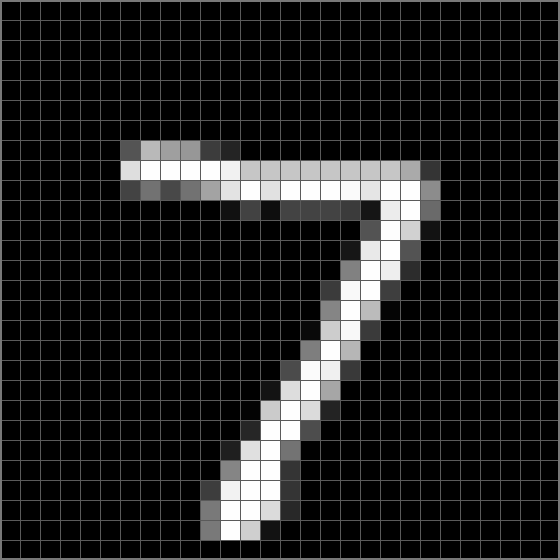
\includegraphics[width=1.32cm]{figures/mnist_digit7.png}};
  % ---------- stack 1: conv+ReLU, 4 maps
  \foreach \k in {3,2,1,0} \draw[orange!85!black,fill=orange!12] (2.9+0.2*\k,-0.9+0.2*\k) rectangle ++(1.8,1.8);
  % ---------- stack 2: pool, 4 maps
  \foreach \k in {3,2,1,0} \draw[orange!85!black,fill=orange!25] (6.0+0.2*\k,-0.5+0.2*\k) rectangle ++(1.0,1.0);
  % ---------- stack 3: conv+ReLU, 8 maps
  \foreach \k in {7,...,0} \draw[red!75!black,fill=red!8] (8.3+0.12*\k,-0.45+0.12*\k) rectangle ++(0.9,0.9);
  % ---------- stack 4: pool, 8 maps
  \foreach \k in {7,...,0} \draw[red!75!black,fill=red!20] (10.4+0.12*\k,-0.25+0.12*\k) rectangle ++(0.5,0.5);
  % ---------- flatten + fully connected
  \foreach \y in {-1.2,-0.8,...,1.6} \fill[gray] (12.4,\y) circle (2pt);
  \foreach \y in {-0.6,0,0.6,1.2} \fill[blue!70!black] (13.4,\y) circle (2.5pt);
  \foreach \a in {-1.2,-0.8,...,1.6} \foreach \b in {-0.6,0,0.6,1.2} \draw[gray,very thin] (12.4,\a) -- (13.4,\b);
  % ---------- output bars
  \foreach \l/\p/\y in {``7''/0.98/0.9,``1''/0.01/0.3,``9''/0.01/-0.3} {
    \node[anchor=east,font=\footnotesize] at (15.3,\y) {\l};
    \fill[blue!70!black!60] (15.35,\y-0.12) rectangle ++(1.2*\p+0.03,0.24);
    \node[anchor=west,font=\footnotesize] at (15.4+1.2*\p,\y) {\p};
  }
  % ---------- arrows
  \foreach \a/\b in {2.1/2.8,5.4/5.9,7.7/8.2,9.9/10.3,11.9/12.25} \draw[->,thick] (\a,0) -- (\b,0);
  \draw[->,thick] (13.6,0.3) -- (14.3,0.3);
  % ---------- stage labels (top)
  \node[align=center,font=\footnotesize] at (1.0,1.85) {\textbf{image}};
  \node[align=center,font=\footnotesize] at (4.1,2.05) {\textbf{conv + ReLU}\\4 filters $\to$ 4 maps};
  \node[align=center,font=\footnotesize] at (6.8,1.85) {\textbf{pool}};
  \node[align=center,font=\footnotesize] at (9.2,2.05) {\textbf{conv + ReLU}\\8 maps};
  \node[align=center,font=\footnotesize] at (11.0,1.85) {\textbf{pool}};
  \node[align=center,font=\footnotesize] at (13.0,2.05) {\textbf{flatten,}\\\textbf{fully conn.}};
  \node[align=center,font=\footnotesize] at (15.9,1.85) {\textbf{probabilities}};
  % ---------- what is detected (bottom)
  \node[font=\footnotesize,gray!40!black] at (4.1,-1.3) {edges};
  \node[font=\footnotesize,gray!40!black] at (9.2,-1.3) {strokes, corners};
  \draw[decorate,decoration={brace,amplitude=5pt,mirror},gray] (2.9,-1.65) -- (11.9,-1.65)
    node[midway,below=5pt,font=\footnotesize]{feature extractor: learns \emph{what} to look for};
  \draw[decorate,decoration={brace,amplitude=5pt,mirror},gray] (12.2,-1.65) -- (17.2,-1.65)
    node[midway,below=5pt,font=\footnotesize]{classifier};
\end{tikzpicture}}

\vspace{6pt}
\begin{itemize}
\item Each conv layer has \textbf{many filters}, one feature map each
  (vertical edges, curves, textures\dots); for colour images a filter spans
  all 3 colour layers. Each map goes through a \textbf{ReLU}.
\item Stacking: maps get smaller but more numerous, and features build up
  from \emph{edges} to \emph{parts} to \emph{objects}.
\item[$\Rightarrow$] Used for medical imaging, self-driving cars, face
  recognition, satellite images\dots\ More on \textbf{computer vision} in
  \textbf{Week 10}.
\end{itemize}

\end{frame}
%%%%%%%%%%%%%%%%%%%%%%%%%%%%%%%%%%%%%%%%%%%%%%%%%%%%%%%%%%%%%%%%%%%%%%
\begin{frame}[fragile]
\frametitle{Sequences}

\begin{itemize}
\item Many kinds of data are not a grid but an \textbf{ordered sequence},
  of \emph{varying length}:
\end{itemize}

\vspace{4pt}
\centerline{%
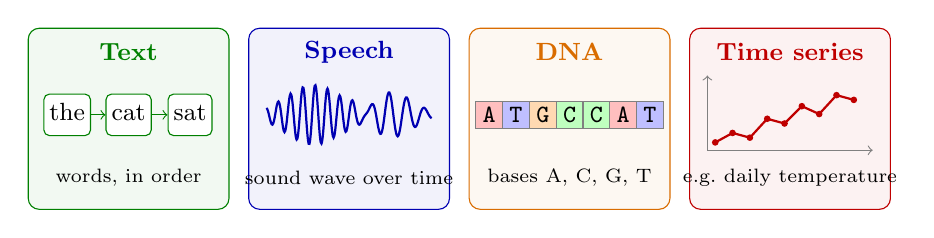
\begin{tikzpicture}[font=\scriptsize,
  card/.style={draw=#1,rounded corners=4pt,fill=#1!5,minimum width=2.55cm,minimum height=2.3cm},
  head/.style={font=\small\bfseries,text=#1}]
  % card frames
  \foreach \k/\col in {0/green!50!black,1/blue!70!black,2/orange!85!black,3/red!75!black}
    \node[card=\col] at (2.8*\k,0) {};
  % ---- Text
  \node[head=green!50!black] at (0,0.85) {Text};
  \foreach \w [count=\i] in {the,cat,sat}
    \node[draw=green!50!black,rounded corners=2pt,fill=white,inner sep=2pt,font=\small] (w\i) at (0.78*\i-1.56,0.05) {\strut\w};
  \foreach \i [evaluate=\i as \j using int(\i+1)] in {1,2} \draw[->,green!50!black] (w\i) -- (w\j);
  \node at (0,-0.75) {words, in order};
  % ---- Speech
  \begin{scope}[shift={(2.8,0)}]
    \node[head=blue!70!black] at (0,0.85) {Speech};
    \draw[blue!70!black,thick,domain=-1.05:1.05,samples=220,smooth]
      plot (\x,{0.05+0.38*exp(-4*(\x+0.45)^2)*sin(2300*\x)+0.28*exp(-7*(\x-0.55)^2)*sin(1600*\x)});
    \node at (0,-0.75) {sound wave over time};
  \end{scope}
  % ---- DNA
  \begin{scope}[shift={(5.6,0)}]
    \node[head=orange!85!black] at (0,0.85) {DNA};
    \foreach \b/\col [count=\i] in {A/red!25,T/blue!25,G/orange!30,C/green!25,C/green!25,A/red!25,T/blue!25}
      \node[draw=gray,fill=\col,inner sep=0pt,minimum size=0.34cm,font=\small\ttfamily] at (0.34*\i-1.36,0.05) {\b};
    \node at (0,-0.75) {bases A, C, G, T};
  \end{scope}
  % ---- Time series
  \begin{scope}[shift={(8.4,0)}]
    \node[head=red!75!black] at (0,0.85) {Time series};
    \draw[gray,->] (-1.05,-0.4) -- (1.05,-0.4);
    \draw[gray,->] (-1.05,-0.4) -- (-1.05,0.55);
    \draw[red!75!black,thick] plot coordinates {(-0.95,-0.3) (-0.73,-0.18) (-0.51,-0.24) (-0.29,0.0) (-0.07,-0.06) (0.15,0.16) (0.37,0.06) (0.59,0.3) (0.81,0.24)};
    \foreach \x/\y in {-0.95/-0.3,-0.73/-0.18,-0.51/-0.24,-0.29/0.0,-0.07/-0.06,0.15/0.16,0.37/0.06,0.59/0.3,0.81/0.24}
      \fill[red!75!black] (\x,\y) circle (1.2pt);
    \node at (0,-0.75) {e.g.\ daily temperature};
  \end{scope}
\end{tikzpicture}}

\vspace{6pt}
\begin{itemize}
\item \textbf{Order matters}: ``dog bites man'' $\neq$ ``man bites dog''.
\item[$\Rightarrow$] We need an architecture that reads the sequence one
  element at a time, carrying forward a \textbf{memory} of what it's seen
  so far: a \textbf{recurrent neural network (RNN)}.
\end{itemize}

\end{frame}
%%%%%%%%%%%%%%%%%%%%%%%%%%%%%%%%%%%%%%%%%%%%%%%%%%%%%%%%%%%%%%%%%%%%%%
\begin{frame}[fragile]
\frametitle{Recurrent neural networks: the core idea}

\begin{itemize}
\item A \textbf{hidden state} $\bs{z}_t$ (a layer of hidden units) is
  updated from the current input $\bs{x}_t$ \emph{and} the previous state:
\[
\bs{z}_t = h\bigl(\bs{W}_{zz}\, \bs{z}_{t-1} + \bs{W}_{xz}\, \bs{x}_t + \bs{b}\bigr),
\qquad \bs{y}_t = f\bigl(\bs{W}_{zy}\, \bs{z}_t\bigr)
\]
\end{itemize}

\centerline{
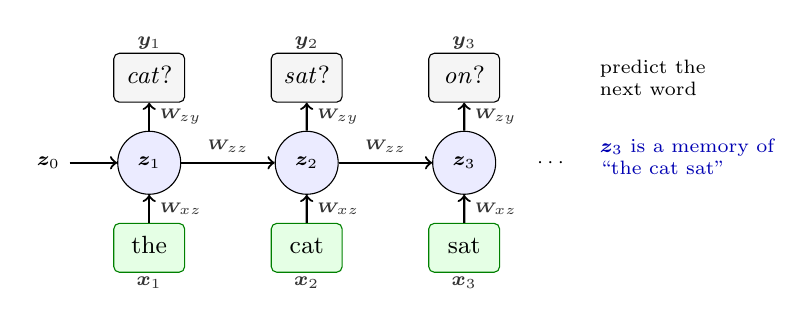
\begin{tikzpicture}[scale=0.8,every node/.style={font=\scriptsize}]
  \node (z0) at (-1.6,0) {$\bs{z}_0$};
  \foreach \i/\x/\w/\p in {1/0/the/cat,2/2.5/cat/sat,3/5.0/sat/on}{
    \node[draw,circle,minimum size=0.8cm,fill=blue!8] (z\i) at (\x,0) {$\bs{z}_{\i}$};
    \node[draw=green!50!black,rounded corners=2pt,fill=green!10,minimum width=0.9cm,minimum height=0.45cm,font=\small] (x\i) at (\x,-1.35) {\strut\w};
    \node[font=\scriptsize,gray!40!black] at (\x,-1.9) {$\bs x_{\i}$};
    \node[draw,rounded corners=2pt,fill=gray!8,minimum width=0.9cm,minimum height=0.45cm,font=\small] (y\i) at (\x,1.35) {\strut\emph{\p}?};
    \node[font=\scriptsize,gray!40!black] at (\x,1.9) {$\bs y_{\i}$};
    \draw[->,thick] (x\i) -- node[right,font=\tiny,gray!40!black]{$\bs W_{xz}$} (z\i);
    \draw[->,thick] (z\i) -- node[right,font=\tiny,gray!40!black]{$\bs W_{zy}$} (y\i);
  }
  \draw[->,thick] (z0) -- (z1);
  \draw[->,thick] (z1) -- node[above,font=\tiny,gray!40!black]{$\bs W_{zz}$} (z2);
  \draw[->,thick] (z2) -- node[above,font=\tiny,gray!40!black]{$\bs W_{zz}$} (z3);
  \node at (6.4,0) {$\cdots$};
  \node[align=left,anchor=west,font=\scriptsize,blue!70!black] at (7.0,0.1) {$\bs z_3$ is a memory of\\``the cat sat''};
  \node[align=left,anchor=west,font=\scriptsize] at (7.0,1.35) {predict the\\next word};
\end{tikzpicture}}

\begin{itemize}
\item Read ``the cat sat'' one word (as a vector $\bs x_t$) at a time;
  after each word, guess the next one.
\item The \emph{same} weight matrices $\bs{W}$ are reused at \emph{every}
  step: \textbf{weight sharing across time}
% \item[$\Rightarrow$] The same backpropagation, applied to the unrolled
  % network (``backpropagation through time'').
\end{itemize}

\end{frame}
%%%%%%%%%%%%%%%%%%%%%%%%%%%%%%%%%%%%%%%%%%%%%%%%%%%%%%%%%%%%%%%%%%%%%%
\begin{frame}[fragile]
\frametitle{RNNs: memory, and its limits}

\begin{itemize}
\item RNNs were the state of the art for translation and speech before 2017.
\end{itemize}

\begin{itemize}
\item But: going back one step, the chain rule \textbf{multiplies} the
  gradient by $\partial \bs z_t/\partial \bs z_{t-1}$:
\end{itemize}

\centerline{%
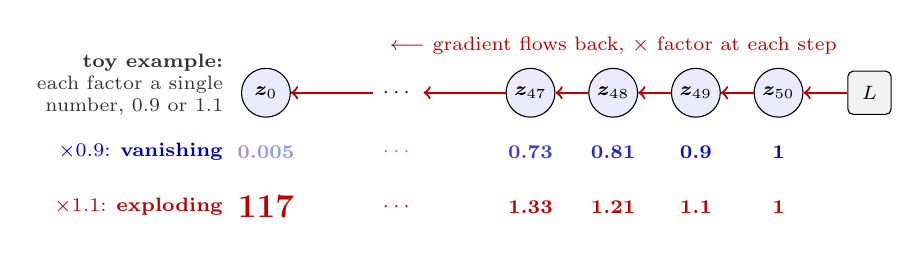
\begin{tikzpicture}[font=\scriptsize,xscale=1.05]
  % chain
  \foreach \lab/\x in {0/0,47/3.2,48/4.2,49/5.2,50/6.2}
    \node[draw,circle,fill=blue!8,inner sep=1pt,minimum size=0.62cm] (n\lab) at (\x,0) {$\bs z_{\lab}$};
  \node (dots) at (1.6,0) {$\cdots$};
  \node[draw,rounded corners=2pt,fill=gray!10,minimum size=0.55cm] (L) at (7.3,0) {$L$};
  \foreach \a/\b in {L/n50,n50/n49,n49/n48,n48/n47} \draw[->,thick,red!75!black] (\a) -- (\b);
  \draw[->,thick,red!75!black] (n47) -- (dots); \draw[->,thick,red!75!black] (dots) -- (n0);
  \node[red!75!black] at (4.2,0.6) {$\longleftarrow$ gradient flows back, $\times$ factor at each step};
  \node[gray!40!black,anchor=east,align=right] at (-0.4,0.1) {\textbf{toy example:}\\each factor a single\\number, 0.9 or 1.1};
  % row labels
  \node[anchor=east,align=right,blue!70!black] at (-0.4,-0.75) {$\times 0.9$: \textbf{vanishing}};
  \node[anchor=east,align=right,red!75!black] at (-0.4,-1.45) {$\times 1.1$: \textbf{exploding}};
  % vanishing values (fading)
  \foreach \x/\v/\o in {0/0.005/0.4,3.2/0.73/0.75,4.2/0.81/0.85,5.2/0.9/0.95,6.2/1/1}
    \node[blue!70!black,opacity=\o] at (\x,-0.75) {\textbf{\v}};
  \node[blue!70!black,opacity=0.5] at (1.6,-0.75) {$\cdots$};
  % exploding values (growing)
  \foreach \x/\v/\f in {3.2/1.33/\scriptsize,4.2/1.21/\scriptsize,5.2/1.1/\scriptsize,6.2/1/\scriptsize}
    \node[red!75!black,font=\f] at (\x,-1.45) {\textbf{\v}};
  \node[red!75!black,font=\large] at (0,-1.45) {\textbf{117}};
  \node[red!75!black] at (1.6,-1.45) {$\cdots$};
\end{tikzpicture}}

\begin{itemize}
\item \textbf{Vanishing gradients}: early words barely affect learning,
  so long-range links are lost.
\item \textbf{Exploding gradients}: huge updates, unstable training.
  % But even they process one step at a time: $\bs{z}_t$ needs $\bs{z}_{t-1}$
  % \emph{first}; no parallelism across the sequence, slow to train.
\end{itemize}

% \begin{itemize}
% \item[$\Rightarrow$] Needed: a way to look \emph{directly} at any earlier
%   token, instead of passing everything along a long chain.
% \end{itemize}

\end{frame}
%%%%%%%%%%%%%%%%%%%%%%%%%%%%%%%%%%%%%%%%%%%%%%%%%%%%%%%%%%%%%%%%%%%%%%
\begin{frame}[fragile]
\frametitle{Why move beyond RNNs?}

\centerline{%
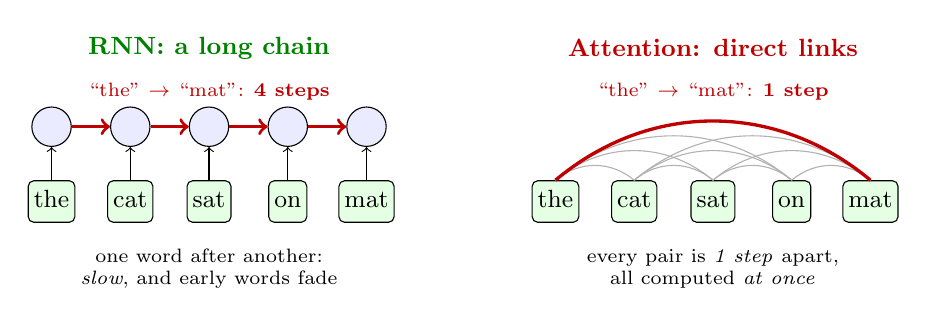
\begin{tikzpicture}[font=\scriptsize,
  wd/.style={draw,rounded corners=2pt,fill=green!10,inner sep=2pt,font=\small}]
  % ---------- RNN panel
  \node[font=\small\bfseries,green!50!black] at (2.0,1.6) {RNN: a long chain};
  \foreach \w/\x [count=\i] in {the/0,cat/1.0,sat/2.0,on/3.0,mat/4.0} {
    \node[draw,circle,fill=blue!8,minimum size=0.5cm,inner sep=0pt] (r\i) at (\x,0.6) {};
    \node[wd] (rw\i) at (\x,-0.35) {\strut\w};
    \draw[->] (rw\i) -- (r\i);
  }
  \foreach \i [evaluate=\i as \j using int(\i+1)] in {1,...,4} \draw[->,very thick,red!75!black] (r\i) -- (r\j);
  \node[red!75!black] at (2.0,1.05) {``the'' $\to$ ``mat'': \textbf{4 steps}};
  \node[align=center] at (2.0,-1.2) {one word after another:\\\emph{slow}, and early words fade};
  % ---------- Attention panel
  \begin{scope}[shift={(6.4,0)}]
    \node[font=\small\bfseries,red!75!black] at (2.0,1.6) {Attention: direct links};
    \foreach \w/\x [count=\i] in {the/0,cat/1.0,sat/2.0,on/3.0,mat/4.0}
      \node[wd] (a\i) at (\x,-0.35) {\strut\w};
    \foreach \i in {1,...,5} \foreach \j in {1,...,5} {
      \ifnum\i<\j \draw[gray!60] (a\i.north) to[bend left=40] (a\j.north); \fi
    }
    \draw[red!75!black,very thick] (a1.north) to[bend left=40] (a5.north);
    \node[red!75!black] at (2.0,1.05) {``the'' $\to$ ``mat'': \textbf{1 step}};
    \node[align=center] at (2.0,-1.2) {every pair is \emph{1 step} apart,\\all computed \emph{at once}};
  \end{scope}
\end{tikzpicture}}

\vspace{6pt}
\begin{itemize}
\item \textbf{Long-range memory}: Vanishing/Exploding gradients. Partial
  fixes exist, e.g.\ the \textbf{LSTM} (\textbf{Long Short-Term Memory},
  Hochreiter \& Schmidhuber, 1997), which adds gates that decide what to
  keep and what to forget.
\item \textbf{Speed}: $\bs z_t$ needs $\bs z_{t-1}$ \emph{first}, so an RNN
  can't process the words in parallel; slow to train on GPUs and large
  datasets.
\item[$\Rightarrow$] Idea: let every word look \emph{directly} at every
  other word, in one step and in parallel: \textbf{attention}.
\end{itemize}

\end{frame}
%%%%%%%%%%%%%%%%%%%%%%%%%%%%%%%%%%%%%%%%%%%%%%%%%%%%%%%%%%%%%%%%%%%%%%
\begin{frame}[fragile]
\frametitle{Self-attention: each word looks at every other word}

\centerline{\large ``The animal didn't cross the street because
\textbf{\color{red!75!black}it} was too tired.''}
\vspace{2pt}
\centerline{What does \emph{it} refer to?}

\vspace{4pt}
\begin{columns}[c]
\begin{column}{0.42\textwidth}
\centerline{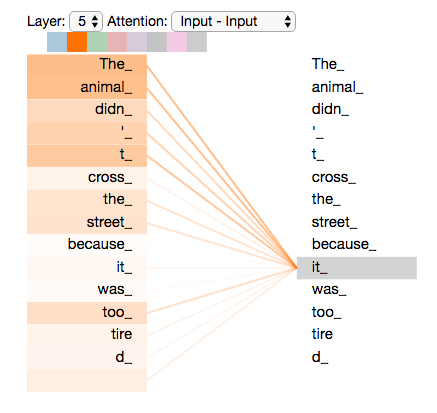
\includegraphics[height=5.3cm]{figures/alammar_self_attention.png}}
\end{column}
\begin{column}{0.56\textwidth}
\begin{itemize}
\item \emph{it} \textbf{attends} to every word; darker $=$ more
  attention, mostly to \emph{The animal}.
\item Its new representation is a \textbf{weighted average} of all the
  words.
\item[$\Rightarrow$] Every word, \emph{directly}, in one step.
\end{itemize}
\end{column}
\end{columns}

\vspace{2pt}
{\fontsize{6}{6}\selectfont Figure: J.\ Alammar, \emph{The Illustrated
Transformer} (2018), CC BY-NC-SA 4.0.\par}

\end{frame}
%%%%%%%%%%%%%%%%%%%%%%%%%%%%%%%%%%%%%%%%%%%%%%%%%%%%%%%%%%%%%%%%%%%%%%
\begin{frame}[fragile]
\frametitle{The attention mechanism}

\small
\begin{itemize}
\item Each word makes three vectors, using learned matrices:
  \begin{itemize}
  \item a {\color{aQ}\textbf{query}}: what it is looking for;
  \item a {\color{aK}\textbf{key}}: what it offers, matched against
    others' queries;
  \item a {\color{aV}\textbf{value}}: the information it passes on if
    matched.
  \end{itemize}
\item Stack them, one row per word, into {\color{aQ}$\bs Q$},
  {\color{aK}$\bs K$}, {\color{aV}$\bs V$}. Then, for all words at once:
\end{itemize}

\vspace{-2pt}
\[
{\color{aZ}\mathsf{Attention}}({\color{aQ}\bs Q}, {\color{aK}\bs K}, {\color{aV}\bs V}) \;=\;
\underbrace{{\color{aS}\mathsf{softmax}}}_{\text{scores}\,\to\,\text{weights}}
\Bigl(\,\underbrace{\frac{{\color{aQ}\bs Q}{\color{aK}\bs K^\top}}{{\color{aS}\sqrt{d_k}}}}_{\text{scaled scores}}\,\Bigr)
\underbrace{{\color{aV}\bs V}}_{\text{values}}
\]

\begin{itemize}
\item {\color{aQ}$\bs Q$}{\color{aK}$\bs K^\top$}: {\color{aS}scores} for every
  (query, key) pair; {\color{aS}$\div\sqrt{d_k}$} keeps them moderate.
\item {\color{aV}$\times\bs V$}: each word's {\color{aZ}output} is a weighted
  average of the {\color{aV}values}.
\end{itemize}

\vspace{2pt}
\setbeamercolor{block title}{bg=aS!15,fg=aS!80!black}
\setbeamercolor{block body}{bg=aS!4}
\begin{block}{Softmax: turning scores into weights}
Scores $s_1,\dots,s_N \;\mapsto\;$ weights
$\alpha_m = \exp(s_m) \big/ \sum_{m'} \exp(s_{m'})$: all positive, sum
to 1, bigger score $\Rightarrow$ bigger weight. \ E.g.\ $(14, 12) \to (0.88, 0.12)$.
\end{block}

\end{frame}
%%%%%%%%%%%%%%%%%%%%%%%%%%%%%%%%%%%%%%%%%%%%%%%%%%%%%%%%%%%%%%%%%%%%%%
\begin{frame}[fragile]
\frametitle{Self-attention step by step}

\begin{columns}[c]
\begin{column}{0.5\textwidth}
\centerline{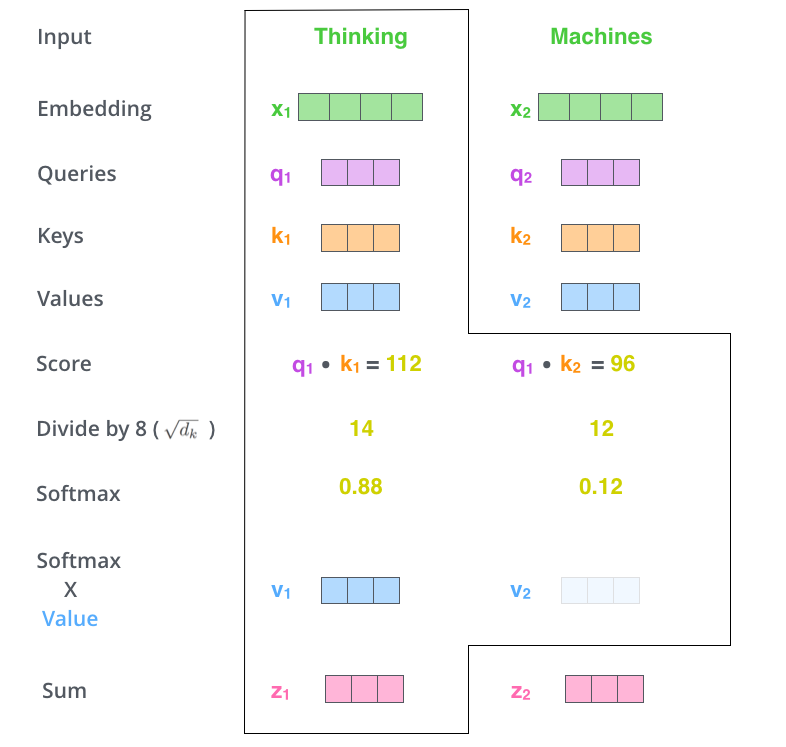
\includegraphics[height=6.1cm]{figures/alammar_self_attention_output.png}}

{\fontsize{6}{6}\selectfont Figure: J.\ Alammar, \emph{The Illustrated
Transformer} (2018), CC BY-NC-SA 4.0.\par}
\end{column}
\begin{column}{0.46\textwidth}
\small
\begin{itemize}
\item By hand, for \emph{Thinking}: {\color{aS}score}
  ({\color{aQ}query}$\cdot${\color{aK}key}) $\to$ {\color{aS}$\div\sqrt{d_k}$}
  $\to$ {\color{aS}softmax} $\to$ weight the {\color{aV}values} $\to$ sum.
\item In vectors, for word $i$:
\[
\begin{aligned}
\alpha_{ij} &= {\color{aS}\mathsf{softmax}_j}\biggl(\frac{{\color{aQ}\bs q_i}\cdot{\color{aK}\bs k_j}}{{\color{aS}\sqrt{d_k}}}\biggr)\\[2pt]
{\color{aZ}\bs z_i} &= \sum\nolimits_{j} \alpha_{ij}\, {\color{aV}\bs v_j}
\end{aligned}
\]
\vspace{-4pt}
\item \textbf{Attention weights} $\alpha_{ij}$: how much attention word $i$
  pays to each word $j$ (here 0.88, 0.12).
\item \textbf{Attention output} {\color{aZ}$\bs z_i$}: the information
  obtained by combining their {\color{aV}values}:\\[2pt]
  \mbox{{\color{aZ}$\bs z_1$} $= 0.88\,{\color{aV}\bs v_1} + 0.12\,{\color{aV}\bs v_2}$}
\end{itemize}
\end{column}
\end{columns}

\end{frame}
%%%%%%%%%%%%%%%%%%%%%%%%%%%%%%%%%%%%%%%%%%%%%%%%%%%%%%%%%%%%%%%%%%%%%%
\begin{frame}[fragile]
\frametitle{Multi-head attention, and positional encoding}

\begin{itemize}
\item \textbf{Multi-head attention}: run several attention computations in
  parallel, each with its \emph{own} learned $\bs{W}_Q,\bs{W}_K,\bs{W}_V$, then combine
  them; one head might learn subject$\leftrightarrow$pronoun links (as
  above), another local word order, another something else entirely, all
  learned rather than specified in advance.
\end{itemize}

\begin{itemize}
\item \textbf{Positional encoding}: attention is a weighted \emph{average}
  over tokens; on its own, it has \textbf{no notion of order} at all.
  Fix: add a position-dependent vector to each token embedding
  \emph{before} attention (fixed, e.g.\ sinusoidal, or learned).
\end{itemize}

\end{frame}
%%%%%%%%%%%%%%%%%%%%%%%%%%%%%%%%%%%%%%%%%%%%%%%%%%%%%%%%%%%%%%%%%%%%%%
\begin{frame}[fragile]
\frametitle{The Transformer: attention is all you need}

\begin{itemize}
\item \textbf{2017} (Vaswani et al.): stack attention blocks into an
  \textbf{encoder} and a \textbf{decoder}; Task: French $\to$ English.
\end{itemize}

\vspace{-2pt}
\centerline{\resizebox{0.92\textwidth}{!}{%
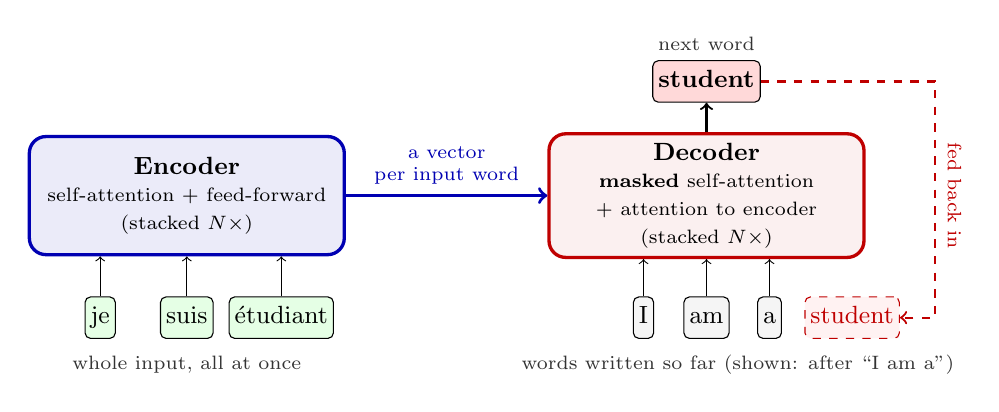
\begin{tikzpicture}[font=\small,
  wd/.style={draw,rounded corners=2pt,inner sep=2pt,minimum height=0.45cm},
  big/.style={draw,rounded corners=6pt,very thick,minimum width=4.0cm,minimum height=1.5cm,align=center}]
  % encoder
  \node[big,draw=blue!70!black,fill=blue!70!black!8] (enc) at (0,0)
    {\textbf{Encoder}\\[-1pt]{\scriptsize self-attention + feed-forward}\\[-1pt]{\scriptsize (stacked $N\times$)}};
  \foreach \w/\x [count=\i] in {je/-1.1,suis/0,{\'etudiant}/1.2} {
    \node[wd,fill=green!10] (in\i) at (\x,-1.55) {\strut\w};
    \draw[->] (in\i) -- (in\i |- enc.south);
  }
  \node[font=\scriptsize,gray!40!black] at (0,-2.15) {whole input, all at once};
  % decoder
  \node[big,draw=red!75!black,fill=red!75!black!6] (dec) at (6.6,0)
    {\textbf{Decoder}\\[-1pt]{\scriptsize \textbf{masked} self-attention}\\[-1pt]{\scriptsize + attention to encoder}\\[-1pt]{\scriptsize (stacked $N\times$)}};
  \foreach \w/\x [count=\i] in {I/5.8,am/6.6,a/7.4} {
    \node[wd,fill=gray!8] (din\i) at (\x,-1.55) {\strut\w};
    \draw[->] (din\i) -- (din\i |- dec.south);
  }
  \node[font=\scriptsize,gray!40!black] at (7.0,-2.15) {words written so far (shown: after ``I am a'')};
  \node[wd,fill=red!15,font=\small\bfseries] (out) at (6.6,1.45) {\strut student};
  \draw[->,thick] (dec) -- (out);
  \node[font=\scriptsize,gray!40!black,anchor=south] at (out.north) {next word};
  % feed-back loop
  \node[wd,dashed,draw=red!75!black,fill=red!5,text=red!75!black] (din4) at (8.45,-1.55) {\strut student};
  \draw[->,dashed,thick,red!75!black] (out.east) -- (9.5,1.45) -- (9.5,-1.55) -- (din4.east);
  \node[font=\scriptsize,red!75!black,rotate=-90] at (9.75,0) {fed back in};

  % link
  \draw[->,very thick,blue!70!black] (enc) -- node[above,font=\scriptsize,align=center]{a vector\\per input word} (dec);
\end{tikzpicture}}}

\vspace{4pt}
\begin{itemize}
\item \textbf{Encoder}: reads the whole input at once; a representation of
  every word, in the context of the others.
\item \textbf{Decoder}: writes one word per step (``I'', ``am'', ``a'',
  ``student'', \textit{end}), each fed back in; looks at its words so far
  \emph{and} the encoder.
\item The decoder uses \textbf{masked (causal) self-attention}: each word
  attends only to itself and \emph{earlier} words; weights on future words
  are set to 0 (no peeking ahead).
\end{itemize}

\end{frame}
%%%%%%%%%%%%%%%%%%%%%%%%%%%%%%%%%%%%%%%%%%%%%%%%%%%%%%%%%%%%%%%%%%%%%%
\begin{frame}[fragile]
\frametitle{Transformer variants: encoder, decoder, or both}

\centerline{%
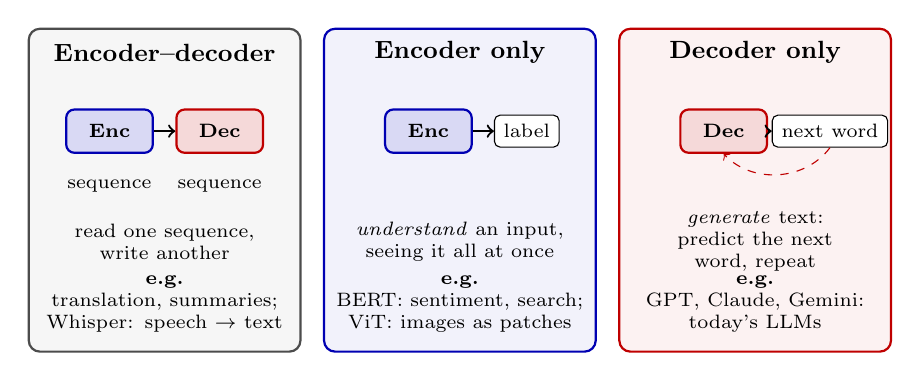
\begin{tikzpicture}[font=\scriptsize,
  card/.style={draw=#1,rounded corners=4pt,thick,fill=#1!5,minimum width=3.45cm,minimum height=4.1cm},
  blk/.style={draw=#1,rounded corners=3pt,thick,fill=#1!15,minimum width=1.1cm,minimum height=0.55cm,font=\scriptsize\bfseries}]
  % ---------- encoder-decoder
  \node[card=gray!60!black] at (0,0) {};
  \node[font=\small\bfseries] at (0,1.75) {Encoder--decoder};
  \node[blk=blue!70!black] (e) at (-0.7,0.75) {Enc};
  \node[blk=red!75!black] (d) at (0.7,0.75) {Dec};
  \draw[->,thick] (e) -- (d);
  \node at (-0.7,0.05) {sequence}; \node at (0.7,0.05) {sequence};
  \node[align=center,text width=3.2cm] at (0,-0.65) {read one sequence,\\write another};
  \node[align=center,text width=3.2cm] at (0,-1.45) {\textbf{e.g.}\\translation, summaries;\\Whisper: speech $\to$ text};
  % ---------- encoder only
  \begin{scope}[shift={(3.75,0)}]
  \node[card=blue!70!black] at (0,0) {};
  \node[font=\small\bfseries] at (0,1.75) {Encoder only};
  \node[blk=blue!70!black] (e2) at (-0.4,0.75) {Enc};
  \node[draw,rounded corners=2pt,fill=white,font=\scriptsize] (lab) at (0.85,0.75) {label};
  \draw[->,thick] (e2) -- (lab);
  \node[align=center,text width=3.2cm] at (0,-0.65) {\emph{understand} an input,\\seeing it all at once};
  \node[align=center,text width=3.2cm] at (0,-1.45) {\textbf{e.g.}\\BERT: sentiment, search;\\ViT: images as patches};
  \end{scope}
  % ---------- decoder only
  \begin{scope}[shift={(7.5,0)}]
  \node[card=red!75!black] at (0,0) {};
  \node[font=\small\bfseries] at (0,1.75) {Decoder only};
  \node[blk=red!75!black] (d3) at (-0.4,0.75) {Dec};
  \node[draw,rounded corners=2pt,fill=white,font=\scriptsize] (nw) at (0.95,0.75) {next word};
  \draw[->,thick] (d3) -- (nw);
  \draw[->,dashed,red!75!black] (nw.south) to[bend left=50] (d3.south);
  \node[align=center,text width=3.2cm] at (0,-0.65) {\emph{generate} text:\\predict the next word, repeat};
  \node[align=center,text width=3.2cm] at (0,-1.45) {\textbf{e.g.}\\GPT, Claude, Gemini:\\today's LLMs};
  \end{scope}
\end{tikzpicture}}

\vspace{6pt}
\begin{itemize}
\item Same building block (self-attention + feed-forward) in all three.
\item[$\Rightarrow$] Decoder-only models, trained on huge amounts of text
  to predict the next word, are the large language models (LLMs) behind
  chatbots.
\end{itemize}

\end{frame}
%%%%%%%%%%%%%%%%%%%%%%%%%%%%%%%%%%%%%%%%%%%%%%%%%%%%%%%%%%%%%%%%%%%%%%
\begin{frame}[fragile]
\frametitle{Where Transformers are used}

\centerline{%
\parbox[t]{0.46\textwidth}{\centering 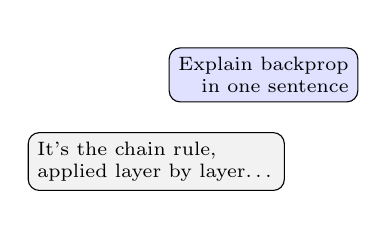
\begin{tikzpicture}[every node/.style={font=\scriptsize}]
  \node[draw,rounded corners,fill=blue!12,anchor=east,align=right] at (4.2,0.5) {Explain backprop\\in one sentence};
  \node[draw,rounded corners,fill=gray!10,anchor=west,align=left] at (0,-0.6) {It's the chain rule,\\applied layer by layer\dots};
  \path (0,1.1) -- (0,-1.35);
\end{tikzpicture}\\[3pt]{\small \textbf{Chatbots and LLMs}: ChatGPT, Gemini, Claude}}
\hspace{0.03\textwidth}
\parbox[t]{0.46\textwidth}{\centering 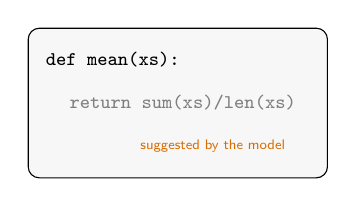
\begin{tikzpicture}[every node/.style={font=\scriptsize\ttfamily,anchor=west}]
  \draw[rounded corners,fill=gray!6] (-0.1,-1.15) rectangle (3.7,0.75);
  \node at (0,0.35) {def mean(xs):};
  \node[gray] at (0.3,-0.2) {return sum(xs)/len(xs)};
  \node[font=\tiny\sffamily,orange!85!black] at (1.2,-0.75) {suggested by the model};
\end{tikzpicture}\\[3pt]{\small \textbf{Code assistants}: suggesting the next lines}}}

\vspace{6pt}
\centerline{%
\parbox[t]{0.46\textwidth}{\centering 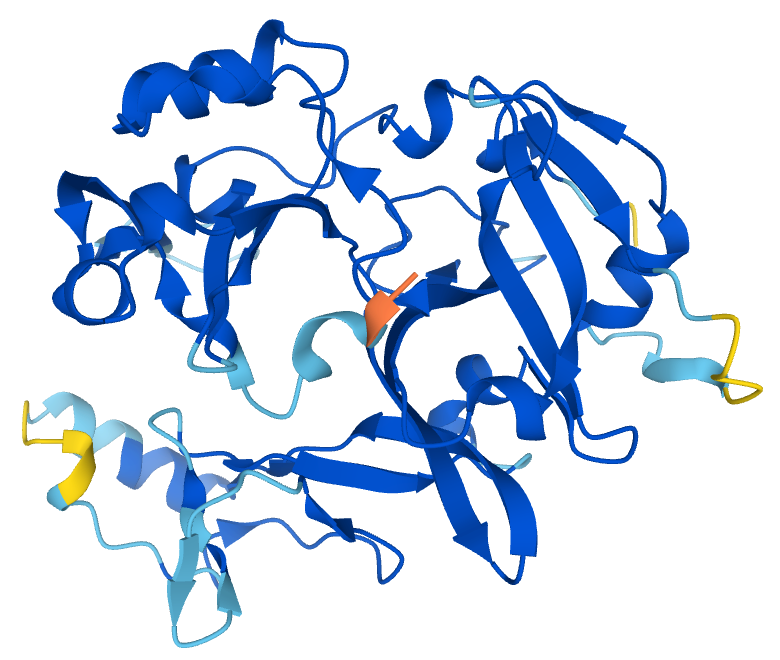
\includegraphics[height=1.6cm]{figures/protein.png}\\[3pt]{\small \textbf{Science}: AlphaFold predicts protein structures}}
\hspace{0.03\textwidth}
\parbox[t]{0.46\textwidth}{\centering 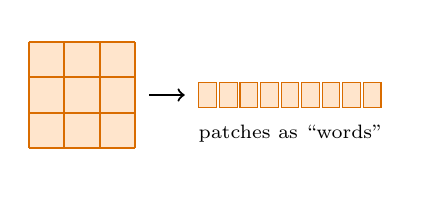
\begin{tikzpicture}[scale=0.45]
  \fill[orange!20] (0,0) rectangle (3,3);
  \draw[step=1,orange!85!black,thick] (0,0) grid (3,3);
  \draw[->,thick] (3.4,1.5) -- (4.4,1.5);
  \foreach \i in {0,...,8} \draw[orange!85!black,fill=orange!20] (4.8+\i*0.58,1.15) rectangle (5.3+\i*0.58,1.85);
  \node[font=\scriptsize] at (7.4,0.4) {patches as ``words''};
  \path (0,-0.8) -- (0,3.4);
\end{tikzpicture}\\[3pt]{\small \textbf{Vision (ViT)}: image classification, image captioning}}}

{\fontsize{6}{6}\selectfont Image: human C12orf29 protein structure predicted
by AlphaFold. CSBIOPASSION, Wikimedia Commons, CC BY-SA 4.0. Method: Jumper
et al., \emph{Nature} (2021).}

\end{frame}
%%%%%%%%%%%%%%%%%%%%%%%%%%%%%%%%%%%%%%%%%%%%%%%%%%%%%%%%%%%%%%%%%%%%%%
\begin{frame}[fragile]
\frametitle{The story so far}

\centerline{\resizebox{\textwidth}{!}{%
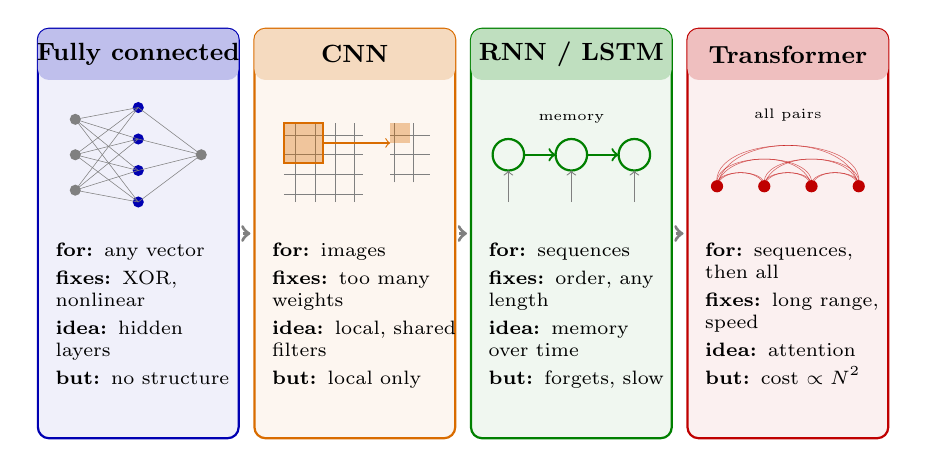
\begin{tikzpicture}
  \begin{scope}[xshift=0cm]
    \draw[rounded corners,thick,blue!70!black,fill=blue!70!black!6] (0,0) rectangle (2.55,5.2);
    \fill[blue!70!black!25,rounded corners] (0,4.55) rectangle (2.55,5.2);
    \node[font=\small\bfseries] at (1.275,4.875) {Fully connected};
    \begin{scope}[shift={(1.275,3.6)}]
      \foreach \y in {-0.45,0,0.45} \fill[gray] (-0.8,\y) circle (2pt);
      \foreach \y in {-0.6,-0.2,0.2,0.6} \fill[blue!70!black] (0,\y) circle (2pt);
      \fill[gray] (0.8,0) circle (2pt);
      \foreach \a in {-0.45,0,0.45} \foreach \b in {-0.6,-0.2,0.2,0.6} \draw[gray,very thin] (-0.8,\a) -- (0,\b);
      \foreach \b in {-0.6,-0.2,0.2,0.6} \draw[gray,very thin] (0,\b) -- (0.8,0);
    \end{scope}
    \node[align=left,font=\scriptsize,text width=2.35cm,anchor=north west] at (0.1,2.6) {\hyphenpenalty=10000\exhyphenpenalty=10000 \textbf{for:} any vector\\[2pt]\textbf{fixes:} XOR, nonlinear\\[2pt]\textbf{idea:} hidden layers\\[2pt]\textbf{but:} no structure};
  \end{scope}
  \begin{scope}[xshift=2.75cm]
    \draw[rounded corners,thick,orange!85!black,fill=orange!85!black!6] (0,0) rectangle (2.55,5.2);
    \fill[orange!85!black!25,rounded corners] (0,4.55) rectangle (2.55,5.2);
    \node[font=\small\bfseries] at (1.275,4.875) {CNN};
    \begin{scope}[shift={(1.275,3.6)}]
      \draw[step=0.25,gray] (-0.9,-0.6) grid (0.1,0.4);
      \fill[orange!85!black,opacity=0.35] (-0.9,-0.1) rectangle (-0.4,0.4);
      \draw[orange!85!black,thick] (-0.9,-0.1) rectangle (-0.4,0.4);
      \draw[->,orange!85!black] (-0.4,0.15) -- (0.45,0.15);
      \draw[step=0.25,gray] (0.45,-0.35) grid (0.95,0.4);
      \fill[orange!85!black,opacity=0.35] (0.45,0.15) rectangle (0.7,0.4);
    \end{scope}
    \node[align=left,font=\scriptsize,text width=2.35cm,anchor=north west] at (0.1,2.6) {\hyphenpenalty=10000\exhyphenpenalty=10000 \textbf{for:} images\\[2pt]\textbf{fixes:} too many weights\\[2pt]\textbf{idea:} local, shared filters\\[2pt]\textbf{but:} local only};
  \end{scope}
  \begin{scope}[xshift=5.5cm]
    \draw[rounded corners,thick,green!50!black,fill=green!50!black!6] (0,0) rectangle (2.55,5.2);
    \fill[green!50!black!25,rounded corners] (0,4.55) rectangle (2.55,5.2);
    \node[font=\small\bfseries] at (1.275,4.875) {RNN / LSTM};
    \begin{scope}[shift={(1.275,3.6)}]
      \foreach \x in {-0.8,0,0.8} \draw[green!50!black,thick] (\x,0) circle (0.2);
      \draw[->,green!50!black,thick] (-0.6,0) -- (-0.2,0);
      \draw[->,green!50!black,thick] (0.2,0) -- (0.6,0);
      \foreach \x in {-0.8,0,0.8} {\draw[->,gray] (\x,-0.6) -- (\x,-0.2);}
      \node[font=\tiny] at (0,0.45) {memory};
    \end{scope}
    \node[align=left,font=\scriptsize,text width=2.35cm,anchor=north west] at (0.1,2.6) {\hyphenpenalty=10000\exhyphenpenalty=10000 \textbf{for:} sequences\\[2pt]\textbf{fixes:} order, any length\\[2pt]\textbf{idea:} memory over time\\[2pt]\textbf{but:} forgets, slow};
  \end{scope}
  \begin{scope}[xshift=8.25cm]
    \draw[rounded corners,thick,red!75!black,fill=red!75!black!6] (0,0) rectangle (2.55,5.2);
    \fill[red!75!black!25,rounded corners] (0,4.55) rectangle (2.55,5.2);
    \node[font=\small\bfseries] at (1.275,4.875) {Transformer};
    \begin{scope}[shift={(1.275,3.6)}]
      \foreach \x [count=\i] in {-0.9,-0.3,0.3,0.9} \fill[red!75!black] (\x,-0.4) circle (2.2pt);
      \foreach \a in {-0.9,-0.3,0.3,0.9} \foreach \b in {-0.9,-0.3,0.3,0.9} \draw[red!75!black,very thin,opacity=0.6] (\a,-0.4) to[out=80,in=100] (\b,-0.4);
      \node[font=\tiny] at (0,0.5) {all pairs};
    \end{scope}
    \node[align=left,font=\scriptsize,text width=2.35cm,anchor=north west] at (0.1,2.6) {\hyphenpenalty=10000\exhyphenpenalty=10000 \textbf{for:} sequences, then all\\[2pt]\textbf{fixes:} long range, speed\\[2pt]\textbf{idea:} attention\\[2pt]\textbf{but:} cost $\propto N^2$};
  \end{scope}
  \foreach \x in {2.6,5.35,8.1} \draw[->,very thick,gray] (\x,2.6) -- (\x+0.1,2.6);
\end{tikzpicture}}}

\end{frame}
%%%%%%%%%%%%%%%%%%%%%%%%%%%%%%%%%%%%%%%%%%%%%%%%%%%%%%%%%%%%%%%%%%%%%%
\begin{titledslide}{Reading}

  \small
  \begin{itemize}
  \item \textbf{Textbook}: Bishop \& Bishop, \emph{Deep Learning: Foundations
    and Concepts} (2024), Ch.\ 10 (convolutional networks) and Ch.\ 12
    (transformers). 
  \item \textbf{CNNs}: Schovia (S.\ Ghanta), ``How AI Sees: A Visual Guide to
    Convolutional Neural Networks'', YouTube, 12 min,
    \href{https://www.youtube.com/watch?v=n0QkWmOFnjs}{youtube.com/watch?v=n0QkWmOFnjs}.
  \item \textbf{RNNs}: StatQuest (J.\ Starmer), ``Recurrent Neural Networks
    (RNNs), Clearly Explained!!!'', YouTube, 17 min,
    \href{https://www.youtube.com/watch?v=AsNTP8Kwu80}{youtube.com/watch?v=AsNTP8Kwu80}
  \item \textbf{Transformers}: J.\ Alammar, \emph{The Illustrated
    Transformer} (2018),
    \href{https://jalammar.github.io/illustrated-transformer/}{jalammar.github.io/illustrated-transformer}
    (highly recommended; source of our attention figures).
  \end{itemize}

\end{titledslide}
%%%%%%%%%%%%%%%%%%%%%%%%%%%%%%%%%%%%%%%%%%%%%%%%%%%%%%%%%%%%%%%%%%%%%%
\end{document}
